Integrated resource system's rated active power = 285 MW as measured at the Connection Point.

While operating at any level of active power output and at any voltage at the Connection Point within the limits of ±10\% of Normal Voltage, the integrated resource system is capable of supplying and absorbing at the Connection Point an amount of reactive power at least equal to the product of the rated active power of the integrated resource system and 0.395, as reflected in Figure 1.

\begin{figure}[H]
	\centering
	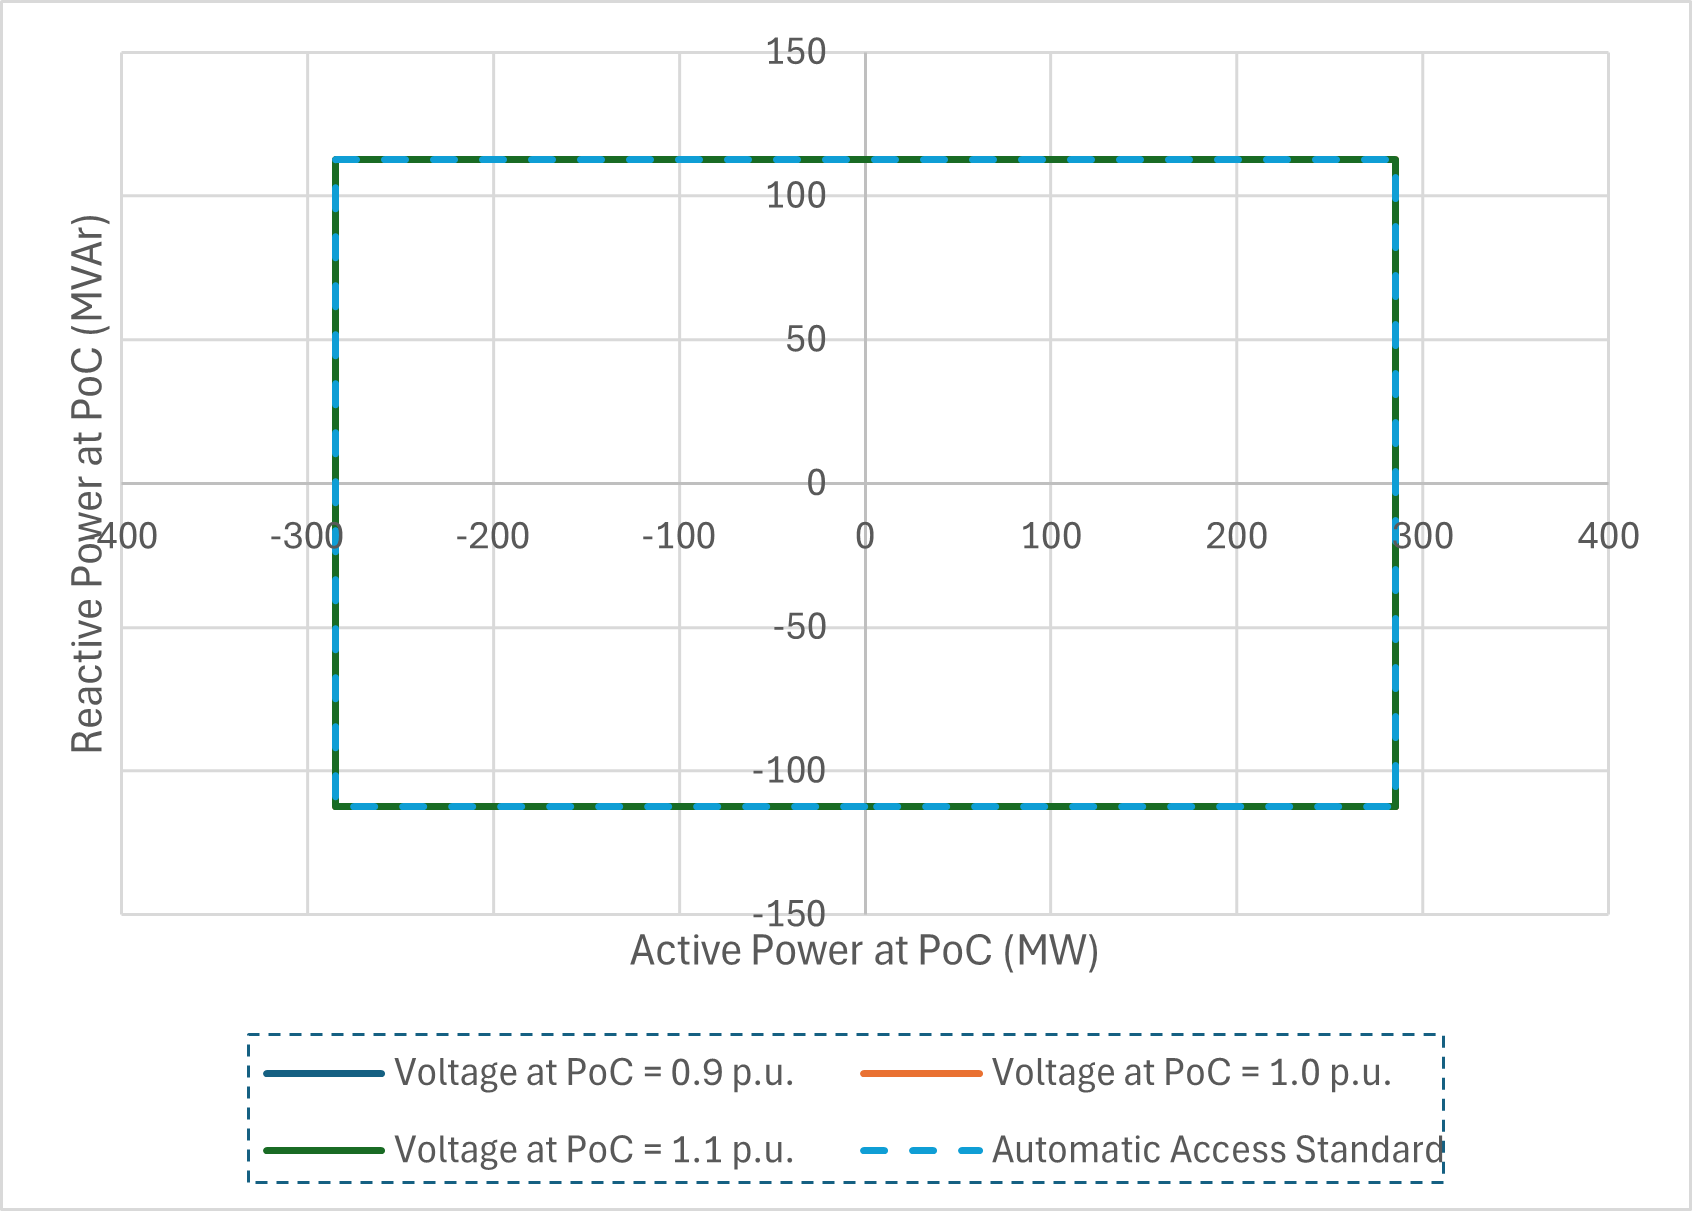
\includegraphics[width=0.8\textwidth]{\projectassetsdir/gps-clauses/s5251-curve.png}
\end{figure}
\textbf{Figure 1: Reactive power capability up to 50°C rating}

The integrated resource system, while not generating active power and not supplying or absorbing reactive power under an ancillary services agreement:
\begin{itemize}
	\item When the production units are connected and the ambient temperature is less than 50OC, follow the voltage regulation control requirement specified in the performance standard under clause S5.2.5.13 with a reactive power capability of ± 1.223 MVAr for each production unit; and
	\item When the production units are not connected, not supply at its Connection Point reactive power of more than 0 MVAr and not draw more electricity than XXXX kW of active power and XXXX kVAr of reactive power;
\end{itemize}

If the reactive power supplied or absorbed at the Connection Point falls outside the range that applies when the production units are not connected, the integrated resource system must, where required by the NSP in order to maintain satisfactory voltage levels at the Connection Point or to restore intra-regional or inter-regional power transfer capability, take action to ensure that the reactive power falls within that range within 30 min.
